\id{IRSTI 81.93.29}{}

\begin{articleheader}
\sectionwithauthors{A.K. Shegetaeva, N.S. Smakova, A.D. Tulegulov, A. Sterenhartz}{ALGORITHM FOR MULTI-FACTORED FORECASTING OF NETWORK VULNERABILITIES: FROM CVE DATA ANALYSIS TO THE DEVELOPMENT OF A FORECASTING MODEL}

{\bfseries
\textsuperscript{1}A.K. Shegetaeva\textsuperscript{\envelope },
\textsuperscript{2}N.S. Smakova,
\textsuperscript{2}A.D. Tulegulov,
\textsuperscript{3}A. Sterenhartz
}
\end{articleheader}

\begin{affiliation}
\textsuperscript{1} Eurasian National University named after L. N. Gumilyov, Astana, Kazakhstan,

\textsuperscript{2} Kazakh University of Technology and Business, Astana, Kazakhstan,

\textsuperscript{3}Technical University of Berlin, Berlin, Germany

\raggedright \textsuperscript{\envelope }Corresponding-author: aizhanshegetaeva@mail.ru
\end{affiliation}

This paper presents an algorithm for multi-factored forecasting of
network vulnerabilities based on data analysis from the CVE (Common
Vulnerabilities and Exposures) database. The goal of the research is to
develop and implement a model capable of not only detecting existing
vulnerabilities but also predicting their future occurrence using formal
methods and machine learning. The authors conduct an overview and
comparative analysis of modern forecasting methods, including
statistical approaches, machine learning algorithms (specifically Random
Forest), clustering, and artificial intelligence methods. As part of the
study, a forecasting program was developed, which uses data on
vulnerability types, severity levels (CVSS), software, and the year of
detection. The model, based on the Random Forest algorithm, demonstrated
high forecasting accuracy (94.14\%). The results were visualized in the
form of graphs and charts, reflecting the dynamics and distribution of
vulnerabilities by year and software categories. The results of the work
confirm the effectiveness of the proposed approach and demonstrate its
potential application in cybersecurity systems for early threat
detection. In the future, it is planned to integrate more complex
models, account for new factors, and create a system for automatic
threat notifications.

{\bfseries Keywords:} multi-factored forecasting algorithm, network
vulnerabilities, forecasting methods, CVSS, CVE, machine learning

\begin{articleheader}
{\bfseries ЖЕЛІ ОСАЛДЫҚТАРЫН КӨП ФАКТОРЛЫ БОЛЖАУ: CVE ДЕРЕКТЕРІН ТАЛДАУМЕН БОЛЖАУ МОДЕЛІН ӘЗІРЛЕУ}

{\bfseries
\textsuperscript{1}А.К. Шегетаева\textsuperscript{\envelope },
\textsuperscript{2}Н.С. Смакова,
\textsuperscript{2}А.Д. Тулегулов,
\textsuperscript{3}А. Штеренхарц
}
\end{articleheader}

\begin{affiliation}
\textsuperscript{1}Л.Н. Гумилев атындағы Еуразия ұлттық университеті, Астана, Қазақстан,

\textsuperscript{2}Қ.Құлажанова атындағы Қазақ технология және бизнес университеті, Астана, Қазақстан,

\textsuperscript{3}Берлин техникалық университеті, Берлин, Германия,

e-mail: \href{mailto:aizhanshegetaeva@mail.ru}{\nolinkurl{aizhanshegetaeva@mail.ru}}
\end{affiliation}

Мақалада CVE (Common Vulnerabilities and Exposions) дерекқорынан алынған
деректерді талдау негізінде желілік осалдықтарды көп факторлы болжау
алгоритмі берілген. Зерттеудің мақсаты -- бар осалдықтарды анықтап қана
қоймай, формальды әдістер мен машиналық оқытуды қолдана отырып, олардың
болашақта пайда болуын болжай алатын модельді әзірлеу және енгізу.
Авторлар статистикалық тәсілдер, машиналық оқыту алгоритмдері (атап
айтқанда, Random Forest), кластерлеу және жасанды интеллект әдістерін
қоса алғанда, қазіргі заманғы болжау әдістеріне шолу мен салыстырмалы
талдау жасайды. Зерттеу осалдық түрлері, ауырлық рейтингтері (CVSS),
бағдарламалық қамтамасыз ету және ашылған жылы туралы деректерді
пайдалана отырып болжау бағдарламасын әзірледі. Кездейсоқ орман
алгоритміне негізделген модель болжамның жоғары дәлдігін көрсетті
(94,14\%). Нәтижелер жыл және бағдарламалық жасақтама категориясы
бойынша осалдықтардың динамикасы мен таралуын көрсететін графиктер мен
диаграммалар түрінде көрнекі түрде көрсетілді. Жұмыстың нәтижелері
ұсынылған тәсілдің тиімділігін растайды және оны қауіптерді ертерек
ескерту үшін киберқауіпсіздік жүйелерінде қолдану әлеуетін көрсетеді.
Болашақта күрделі модельдерді біріктіру, жаңа факторларды есепке алу
және қауіптер туралы автоматты түрде хабарлау жүйесін құру жоспарлануда.

{\bfseries Түйін сөздер:} көп нұсқалы болжау алгоритмі, желінің
осалдықтары, болжау әдістері, CVSS, CVE, машиналық оқыту

\begin{articleheader}
{\bfseries АЛГОРИТМ МНОГОФАКТОРНОГО ПРОГНОЗИРОВАНИЯ СЕТЕВЫХ УЯЗВИМОСТЕЙ: ОТ
АНАЛИЗА ДАННЫХ CVE К РАЗРАБОТКЕ МОДЕЛИ ПРОГНОЗИРОВАНИЯ}

{\bfseries
\textsuperscript{1}А.К. Шегетаева\textsuperscript{\envelope },
\textsuperscript{2}Н.С. Смакова,
\textsuperscript{2}А.Д. Тулегулов,
\textsuperscript{3}А. Штеренхарц
}
\end{articleheader}

\begin{affiliation}
\textsuperscript{1}Евразийский национальный университет им. Л.Н. Гумилева, Астана, Казахстан,

\textsuperscript{2}Казахский университет технологии и бизнеса им. К. Кулажанова, Астана, Казахстан,

\textsuperscript{3}Берлинский технический университет, Берлин, Германия,

e-mail: \href{mailto:aizhanshegetaeva@mail.ru}{\nolinkurl{aizhanshegetaeva@mail.ru}}
\end{affiliation}

В статье представлен алгоритм многофакторного прогнозирования сетевых
уязвимостей на основе анализа данных из базы CVE (Common Vulnerabilities
and Exposures). Цель исследования заключается в разработке и внедрении
модели, способной не только выявлять существующие уязвимости, но и
предсказывать их появление в будущем с применением формальных методов и
машинного обучения. Авторы проводят обзор и сравнительный анализ
современных методов прогнозирования, включая статистические подходы,
алгоритмы машинного обучения (в частности, Random Forest), кластеризацию
и методы искусственного интеллекта. В рамках исследования была
разработана программа прогнозирования, использующая данные о типах
уязвимостей, степени критичности (CVSS), программном обеспечении и годе
обнаружения. Модель, основанная на алгоритме случайного леса, показала
высокую точность прогнозирования (94,14\%). Проведена визуализация
результатов в виде графиков и диаграмм, отражающих динамику и
распределение уязвимостей по годам и категориям программного
обеспечения. Результаты работы подтверждают эффективность предложенного
подхода и демонстрируют потенциал его применения в системах
кибербезопасности для раннего предупреждения угроз. В перспективе
планируется интеграция более сложных моделей, учет новых факторов и
создание системы автоматического уведомления об угрозах.

{\bfseries Ключевые слова:} алгоритм многофакторного прогнозирования,
сетевые уязвимости, методы прогнозирования, CVSS, CVE, машинное обучение

\begin{multicols}{2}
{\bfseries Introduction.} In today' s world, network
infrastructure security is becoming one of the key challenges for
organizations. Network vulnerabilities are a serious threat that can
lead to unauthorized access to data and leakage of confidential
information. Predicting these vulnerabilities helps to identify possible
threats in a timely manner and significantly reduce risks for
organizations and users. Currently, one of the best known vulnerability
databases is the National Vulnerability Database (NVD)
(\url{https://nvd.nist.gov/}) {[}1{]}, a popular knowledge base
consisting of the Common Vulnerability and Exposures (CVE)
(\url{https://www.cve.org/}) {[}2{]} and Common Vulnerability Scoring
System (CVSS) {[}3{]} vocabulary that assesses the impact of these
vulnerabilities. Network vulnerabilities can include flaws in protocols,
misconfigured network devices, and open ports. These issues can be
exploited by attackers to gain unauthorized access to systems.

A significant portion --- arguably the main one --- is devoted to
studies addressing various issues of computer network security, as
networks continue to be the primary source of attacks and network
traffic remains the main vector for penetration and exploit delivery
{[}4{]}.

Thus, it is important for researchers and system administrators to
identify network vulnerabilities in a timely manner, analyze them, and
initiate appropriate countermeasures. In this context, various publicly
available vulnerability databases such as CVE and NVD play a key role in
vulnerability analysis and prediction. They collect, structure and
prepare information on published vulnerabilities.

This paper discusses the use of formal prediction methods to analyze
vulnerabilities and develop a program that uses actual data from the CVE
database. This will not only identify existing vulnerabilities, but also
predict their future occurrence, which is an important step in ensuring
security.

The main objective of the research is to develop and implement a model
of network vulnerability prediction algorithm based on formal methods
using retrospective data from CVE database. To achieve this goal,
several tasks need to be accomplished:

1. Studying existing formal prediction methods applicable to the field
of information security.

2. Analyzing data from the CVE database to identify patterns and trends
in vulnerabilities.

3. Developing a program capable of predicting the occurrence of
vulnerabilities based on actual data.

4. Evaluating the accuracy and effectiveness of the proposed model for
vulnerability prediction.

These tasks will help to create a reliable tool for analysis and
prediction, which will improve the security level of information
systems.

{\bfseries Materials and methods.} Forecasting is an important tool in
scientific research, including information security. As a result, data
storage should be secured to avoid any threats that may cause attacks
{[}5{]}. The most common forecasting methods are divided into several
groups:

- statistical methods (linear regression, time series);

- machine learning (SVM, decision trees, random forest, neural
networks);

- clustering algorithms and associative rules (K-means, DBSCAN);

- artificial intelligence methods (deep learning, genetic algorithms).

Below we analyze the comparison of advantages and disadvantages of using
forecasting methods and sections (Table 1):

Among these methods, we focused on the use of machine learning
techniques, in particular Random Forests, as they allow for efficient
handling of large amounts of data and can be applied to predict
categorical variables such as vulnerability type. This makes them
particularly suitable for our task (Table 1). Machine learning is a type
of artificial intelligence technique that can automatically discover
useful information from massive datasets {[}6{]}.

All vulnerability data was taken from the CVE database and
\url{https://vuldb.com/?archive} {[}7{]}, it contains information about
the identified vulnerabilities, including the following key parameters:

- Year the vulnerability was discovered.

- Criticality level (CVSS score).

- Type of vulnerability (remote access, code execution, etc.).

- Software that is affected by the vulnerability.
\end{multicols}

\tcap{Table 1: Analysis of formal forecasting methods}
\begin{longtblr}[
  label = none,
  entry = none,
]{
  width = \linewidth,
  colspec = {Q[100]Q[121]Q[166]Q[133]Q[187]Q[230]},
  rows = {font = \scriptsize},
  row{1} = {c},
  cell{2}{1} = {r=2}{c},
  cell{2}{2} = {c},
  cell{3}{2} = {c},
  cell{4}{1} = {r=3}{c},
  cell{4}{2} = {c},
  cell{5}{2} = {c},
  cell{6}{2} = {c},
  cell{7}{1} = {r=2}{c},
  cell{7}{2} = {c},
  cell{8}{2} = {c},
  cell{9}{1} = {r=2}{c},
  cell{9}{2} = {c},
  cell{10}{2} = {c},
  vlines,
  hline{1-2,4,7,9,11} = {-}{},
  hline{3,5-6,8,10} = {2-6}{},
}
\textbf{Forecasting methods} & \textbf{Sections			of forecasting methods} & \textbf{Application} & \textbf{Advantages} & \textbf{Disadvantages} & \textbf{In the context of the study}\\
\textbf{Statistical methods} & Linear regression & {
			Basic
			method, but may not account for complex nonlinear analysis
			\\~\\~\\~\\~} & {- easy
				to apply;\\- works
				well with linear relationships between variables\\~} & - does
					not account for interactions between multiple factors, which is
					important in vulnerability prediction where multiple variables
					may interact & Using
			linear regression can produce simple and quick predictions, but
			more sophisticated techniques such as machine learning are
			required for more accurate predictions\\
 & Time series & Analyzes
			the number of network vulnerabilities over time & {- accurate
				forecasts of future values can be made on the basis of historical
				data\\~} & - requires
					a fairly large amount of historical data & The
			use of time series makes it possible to predict how many
			vulnerabilities may appear in the future\\
\textbf{\textbf{Machine learning}} & \textbf{Support			Vector Method (SVM)} & Used
			to categorize types of vulnerabilities & {- efficiently
				small amounts of data and categorizes complex, high-dimensional
				data;\\- Can
				work well with non-linear dependencies\\~} & - Does
					not always scale efficiently with large amounts of data & Useful
			for building classification models, but may be less effective when
			dealing with large datasets and complex features\\
 & \textbf{\textbf{Decision Trees }			} & Represent
			a graphical model where each decision is displayed as a node and
			the results as leaves & - easily
				interpretable & {- Overfitting
				when trees are too complex.\\- Difficulty
					in interpretation for very deep trees} & Random
			Forest shows good results for classifying vulnerability types and
			allows us to identify the importance of features, which is a big
			plus when analyzing data from CVEs\\
 & \textbf{Random Forest} & Allows
			prediction, by type of vulnerability based on retrospective data
			and their characteristics & {- Do
				well with a large number of attributes and categorical data.\\- Can
				work effectively with missing data\\~} & - When
			dealing with very large datasets, a random forest can require a
			lot of memory and processing time & You
			can combine random forest with other approaches for best results\\
\textbf{\textbf{Clustering methods}} & \textbf{\textbf{K-means algorithm}} & Is
			used to group vulnerabilities based on similar characteristics, by
			type of vulnerability or type of attacked software & {- Fast
			and efficient algorithms for clustering.\\- Easily
			scalable to large datasets
		} & {- Requires
			predetermined number of clusters.\\- Not
				always effective for clustering complex and high-dimensional data\\~} & Useful
			for more accurate clustering considering more complex
			dependencies, better to use more advanced methods like DBSCAN\\
 & \textbf{\textbf{DBSCAN (Density-Based Spatial Clustering of Applications with Noise)}} & Used
			for infrequent but highly critical vulnerabilities & {- Does
					not require a predetermined number of clusters.\\- Can
					handle noisy data
		} & {- Requires
				setting two parameters (distance threshold and minimum number of
				points) labor intensive\\~} & Useful
			for identifying rare or unusual vulnerabilities that may be
			particularly dangerous, but its effectiveness depends on the
			quality of the data\\
\textbf{\textbf{Forecasting methods based on artificial intelligence}} & \textbf{\textbf{Deep Learning}} & Is
			used for more sophisticated data analysis, to predict not only the
			type of vulnerability but also potential attack targets, using
			information about software and configurations & {- Can
					process huge amounts of data and identify complex patterns.\\- Works
				well with unstructured data such as textual descriptions of
				vulnerabilities\\~} & {- Require
					large computational resources.\\- It
					is not always easy to interpret the results (black box).} & Significantly
			improves prediction accuracy, especially when the data includes
			unstructured information (textual data from vulnerability
			descriptions), but requires significant computational resources
			and training time\\
 & \textbf{\textbf{Genetic algorithms}} & Used
			to optimize the hyperparameters of a prediction model, in the case
			of machine learning or neural networks & {- Good
					for optimizing complex tasks.\\- Can
					find optimal solutions in large parameter spaces
		} & {- Can
					be time-consuming to find optimal solutions\\- Does
					not always give optimal results for all types of tasks
		} & Are
			useful for model optimization, but are not always suitable for
			predicting vulnerability types because they focus on parameter
			optimization rather than data analysis
\end{longtblr}

{\bfseries Fig.1 - Data from the database \url{https://vuldb.com/?archive}}

\begin{multicols}{2}
For our study we used a set of vulnerability data for further analysis
(see Graph 1).

We study the period from 2010 to 2025, we want to record and analyze the
largest number of network vulnerabilities, as well as assess the
dynamics of vulnerability growth.

As a result of analyzing the data, the main patterns have been
highlighted:

- the highest number of vulnerabilities occurs between 2010 and 2025;

- vulnerabilities related to remote code execution occupy a significant
part among all types of vulnerabilities;

- the degree of vulnerability criticality varies, but vulnerabilities
with high or critical CVSS score remain the most dangerous.

Based on the components of the Common Vulnerability Scoring System
(CVSS) vector, a numerical vulnerability score (CVSS severity score) is
calculated.

The program for vulnerability prediction was developed using machine
learning and statistical analysis methods. The algorithm was built using
the scikit-learn library, which provides many tools for data processing
and model training {[}8{]}.

1. Data preparation:

- vulnerability data were cleaned and processed, including converting
categorical data into numerical values (e.g., criticality and
vulnerability type);

- parameters such as year, vulnerability type, CVSS score, and others
were used as attributes.

2. Model training:

- random Forest algorithm (Random Forest) was used to classify
vulnerability types;

- the model was trained on 70\% of the data and the remaining 30\% was
used for testing.

3. Model Evaluation:

- the model showed good prediction accuracy (about 94\%) on the test
data.

- the importance of attributes was determined and the most influential
parameters were criticality and vulnerability type.
\end{multicols}

\begin{figure}[H]
	\centering
	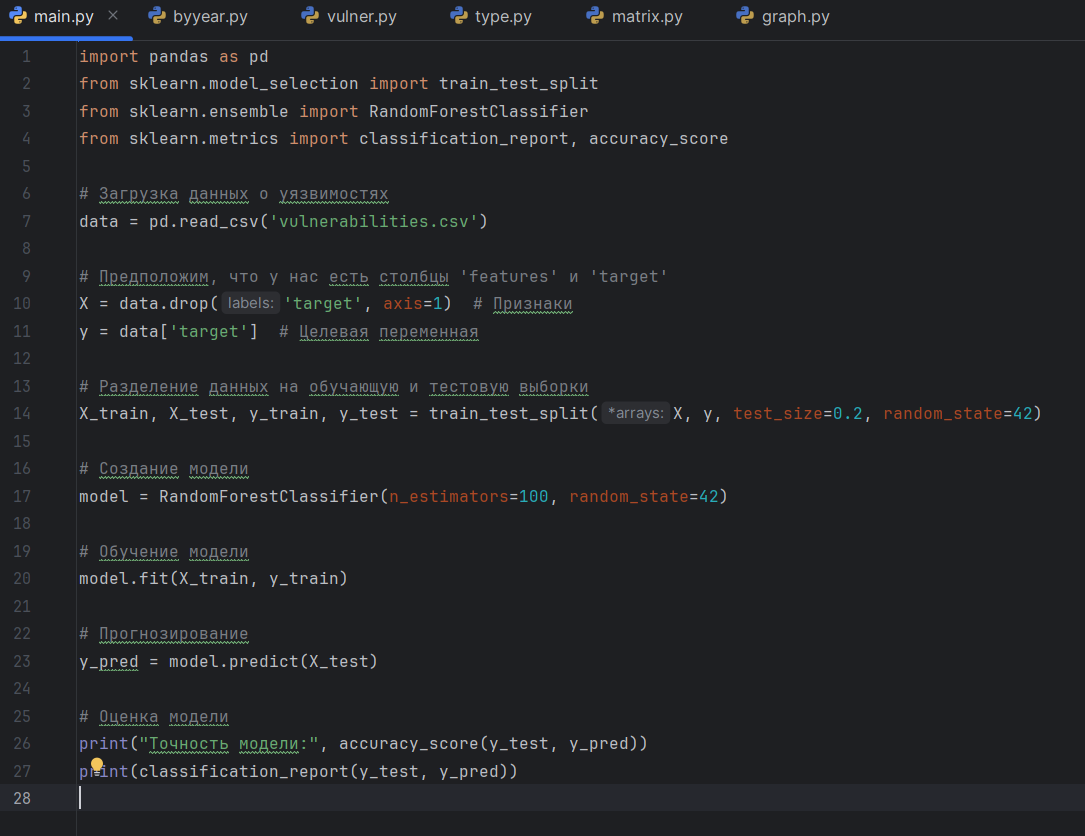
\includegraphics[width=0.8\textwidth]{media/ict2/image165}
	\caption*{Fig.1 - Vulnerability prediction program codes}
\end{figure}

\begin{multicols}{2}
{\bfseries Results and Discussion.} The outcome of the code depends on
several factors, including the data we used to train the model and the
methods used to assess accuracy and predict vulnerabilities. In our
case, the following key points are the results:

1. Predicted data

Based on retrospective CVE data, the model predicts:

- the probability of vulnerabilities occurring in the future, as well as
their nature (type, threat severity, software to be attacked);

- classification of vulnerabilities: what degree of criticality the
vulnerability will be in (``medium criticality'', ``high criticality'').

2. Model Evaluation

The result is evaluated using several metrics such as:

- accuracy: the percentage of correct predictions;

- confusion Matrix: to understand how often the model is wrong and in
what ways;

- precision and Completeness (Precision, Recall): to evaluate the
accuracy of the prediction for each type of vulnerability.

3. The result of the random forest model:

Рython

Accuracy: 94.14\%

This means that on the test data the model was able to correctly predict
the accuracy of the vulnerability in 94.14\% of cases (see Figure 1).

Based on the above research, we present the results of the dynamics of
network vulnerabilities registered in the CVE database in order to
identify trends and predict future threats in the field of information
security:

1) Graph of vulnerability distribution by year (Time Series)

For this purpose, a forecasting model was developed, presented as a
graph illustrating the change in the number of vulnerabilities by year,
which allows us to identify trends and predict a possible increase or
decrease in the number of vulnerabilities in the future.
\end{multicols}

Python

\begin{lstlisting}
import matplotlib.pyplot as plt
import pandas as pd

data = {
    'Year': [2015, 2016, 2017, 2018, 2019, 2020, 2021, 2022, 2023, 2024, 2025],
    'Vulnerabilities': [7231, 8342, 16287, 17523, 18527, 18874, 22786, 27065, 32149, 40111, 14844]
}

df = pd.DataFrame(data)

plt.figure(figsize=(10,6))
plt.plot(df['Year'], df['Vulnerabilities'], marker='o')
plt.title('Distribution of vulnerabilities by year')
plt.xlabel('Years')
plt.ylabel('Number of vulnerabilities')
plt.grid(True)
plt.show()
\end{lstlisting}

{\bfseries Graph 2 - Result of distribution of vulnerabilities by years}

1) Figure 2 illustrates the evolution of the number of network
vulnerabilities registered in the CVE database from 2010 to 2025. The
X-axis shows the years and the Y-axis shows the number of
vulnerabilities identified in each year. The line on the graph shows
an increasing trend in the number of vulnerabilities, indicating an
increase in information security threats. The graph shows that the
highest number of vulnerabilities was recorded in 2024, which may
indicate an increase in the activity of attackers and an increase in
the number of vulnerabilities in software (Graph 2).

2) Vulnerability distribution diagram by type (Pie Chart)
To display the distribution of vulnerabilities by threat type (remote
code execution, data leakage, etc.) we developed a prediction model in
Python:

Python

\begin{lstlisting}
import matplotlib.pyplot as plt
# Vulnerability data
data = {
    "Operating System": 24048
    "WordPress Plugin": 17363
   "Web Browser": 11612,
    "Smartphone OS": 11457,
    "CMS": 10242,
    "Router OS": 4937,
    "Programming Language Software": 4566,
    "Cloud Software": 4457,
    "Database Software": 3938,
    "Other": 0, } # here a data dictionary is created that contains the software categories as keys and the corresponding number of vulnerabilities as values. This is the initial data that will be used to build the graph.
threshold = 3500 # here you set a threshold value (3500) that will be used to filter the data. Vulnerabilities that are less than this threshold will be combined into the "Other" category.
aw_data = {
    "Document Reader Software": 3625,
   "Multimedia Player Software": 3266,
    "Firewall Software": 3245,
    "Image Processing Software": 2789,
    "Chip Software": 2601,
    "Application Server Software": 2562,
    "Virtualization Software": 2536,
    "Groupware Software": 2211,
    "Forum Software": 2165,
    "Bug Tracking Software": 1842,
    "Programming Tool Software": 1831,
    "Anti-Malware Software": 1668,
    "Automation Software": 1648,
    "E-Commerce Management Software": 1625,
    "SCADA Software": 1588,
    "Digital Media Player": 1541,
    "Web Server": 1482,
    "Network Management Software": 1426,
    "Smartwatch OS": 1389,
    "Wireless LAN Software": 1366,
    "Project Management Software": 1306,
    "Log Management Software": 1299,
    "Enterprise Resource Planning Software": 1191,
    "Other": 0, } # another raw_data dictionary is created here, which contains additional software categories and the number of vulnerabilities for each of them. This data will be processed and added to the main data dictionary.

for key, value in raw_data.items():
    if value >= threshold:
        data[key] = value
    else:
        data["Other"] += value # In this loop, the data from raw_data is processed:
# For each category (key) and its number of vulnerabilities (value), it is checked whether the value exceeds the threshold (3500);
# - if the value is greater than or equal to the threshold, it is added to the data dictionary;
# - if the value is less than the threshold, it is added to the value in the “Other” category.
labels = list(data.keys()) # labels: creates a list of labels (software categories) from the keys of the data dictionary.
sizes = list(data.values()) # sizes: creates a list of values (number of vulnerabilities) from the values of the data dictionary.
plt.figure(figsize=(10, 10)) # creates a new shape for the chart with specified dimensions (10 inches by 10 inches)
plt.pie(sizes, labels=labels, autopct='%1.1f%%', startangle=140) # function for drawing a pie chart.
# sizes: values defining the size of the diagram sectors.
# labels: labels for each sector.
autopct='%1.1f%%' # the format for displaying percentages on a chart (one decimal place).
startangle=140: # the angle from which the diagram starts (to improve visual perception).
plt.title("Distribution of vulnerabilities by software category") # sets the title for the graph
plt.show() # graph
\end{lstlisting}

\begin{figure}[H]
	\centering
	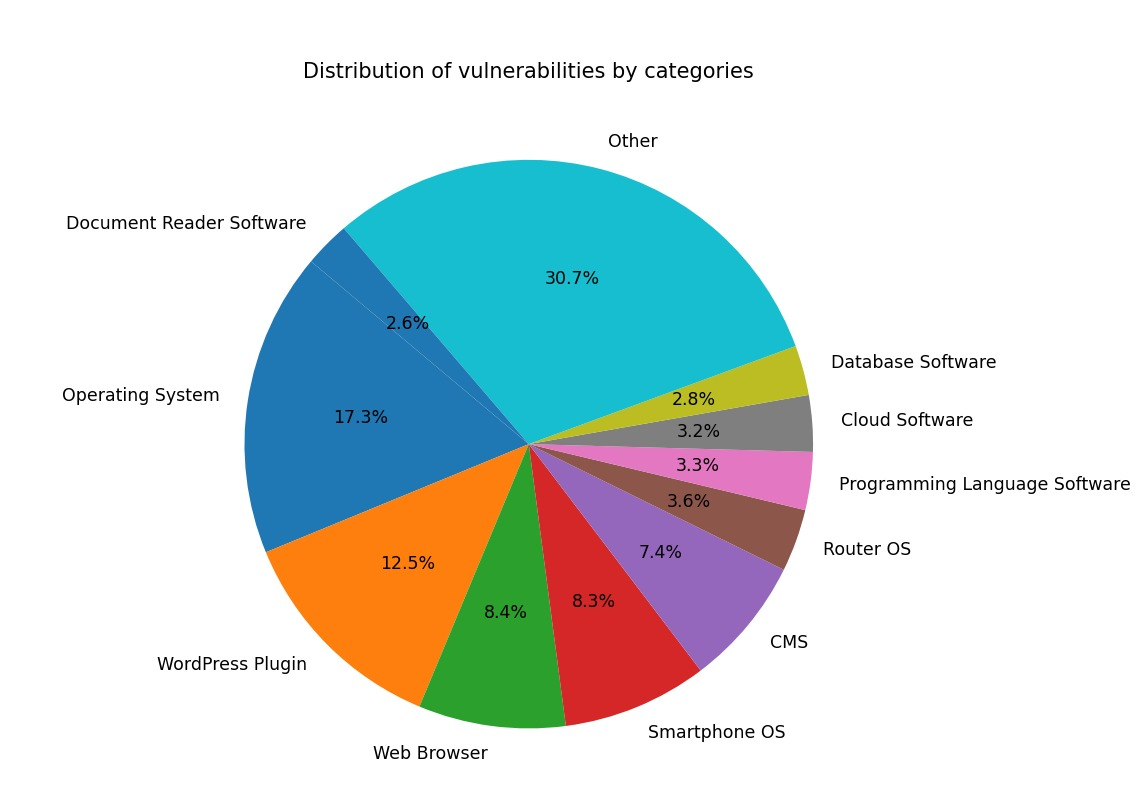
\includegraphics[width=0.8\textwidth]{media/ict2/image166}
	\caption*{Fig.3 - Result of vulnerability distribution by software category}
\end{figure}

\begin{multicols}{2}
3) Figure 3 is a pie chart showing the distribution of network
vulnerabilities across different categories of network vulnerabilities
and software. Each section of the chart corresponds to a specific
category such as ``Operating System'', ``WordPress Plugins'', ``Web
Browsers'', etc. The percentage of each category is displayed on the
chart, allowing you to quickly assess which types of software and
networks are most vulnerable to vulnerabilities. According to the
chart, you can see that the largest number of vulnerabilities are
related to operating systems, which emphasizes the importance of
protecting them (see chart 3).

4) Prediction of vulnerabilities by type with a probability of
For prediction, a model was developed using the Python language,
represented as a histogram that visualizes the probabilities of
different types of vulnerabilities.
\end{multicols}

Python

\begin{lstlisting}
import numpy as np
import matplotlib.pyplot as plt
from sklearn.linear_model import LinearRegression
import os
os.environ["LOKY_MAX_CPU_COUNT"] = '4'
def forecast_vulnerabilities(data):
    # Years from 2010 to 2024
    years = np.array([2010, 2011, 2012, 2013, 2014, 2015, 2016, 2017, 2018, 2019, 2020, 2021, 2022, 2023, 2024]).reshape(-1, 1)
    predictions = {}

    for vuln_type, values in data.items():
        values = np.array(values).reshape(-1, 1)
        model = LinearRegression()
        model.fit(years, values)
        pred_2025 = model.predict([[2025]])[0][0]
        predictions[vuln_type] = max(0, round(pred_2025))
    return predictions
def calculate_percentages(predictions):
    total = sum(predictions.values())
    percentages = {k: round((v / total) * 100, 2) for k, v in predictions.items()}
    threshold = 5.0
    major = {k: v for k, v in percentages.items() if v >= threshold}
    minor = {k: v for k, v in percentages.items() if v < threshold}

    major["Other"] = round(sum(minor.values()), 2)
    return major
\end{lstlisting}

\begin{figure}[H]
	\centering
	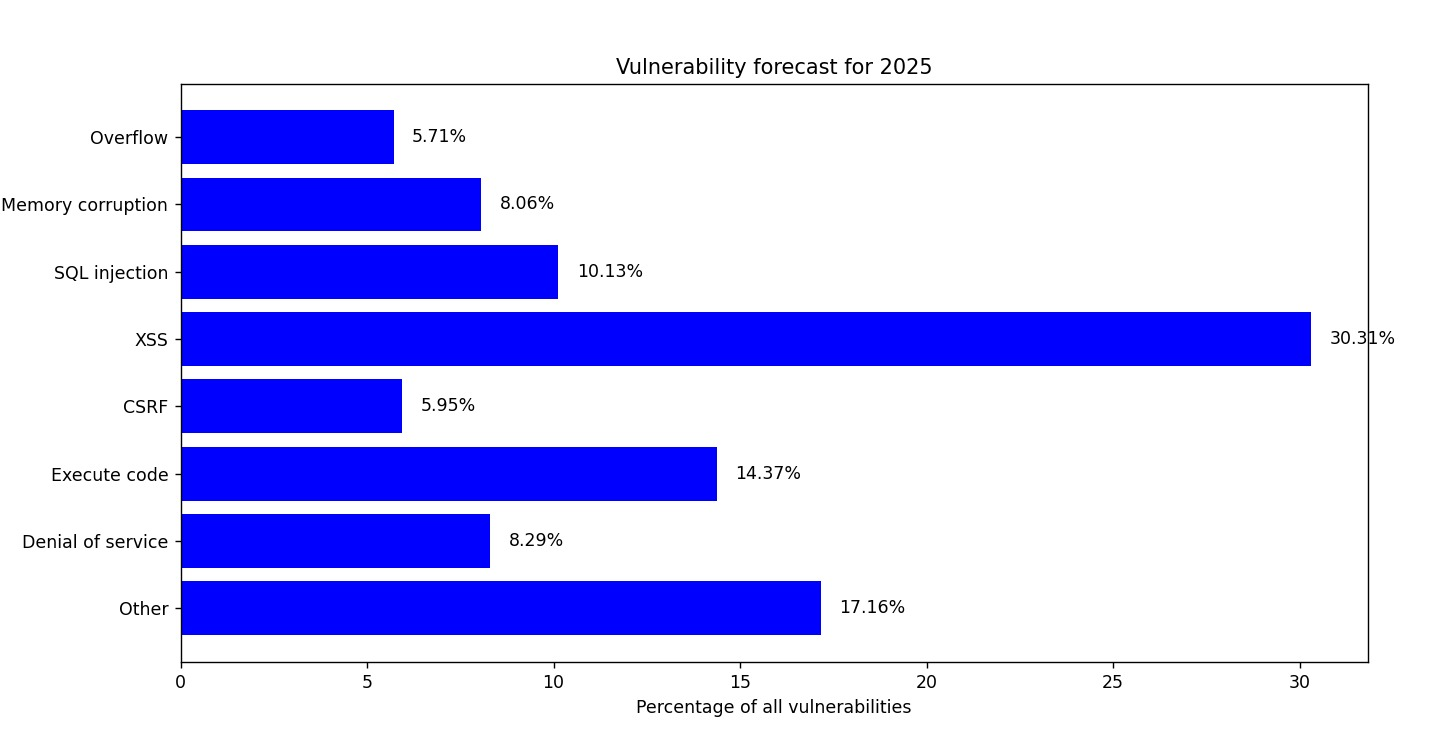
\includegraphics[width=0.8\textwidth]{media/ict2/image167}
	\caption*{Fig.4 - Result of the distribution of predicted vulnerabilities by type as of 2025}
\end{figure}

\begin{multicols}{2}
Figure 4 shows the projected distribution of different types of
vulnerabilities for 2025. The graph shows columns, each corresponding to
a specific type of vulnerability, with their probability of occurrence
in percentages. The graph allows you to visually assess which types of
vulnerabilities, such as Remote Code Execution or Data Leakage, will be
most prevalent in the future. This can help organizations prepare in
advance for potential threats and focus their efforts on protecting the
most vulnerable areas {[}9{]}.

The data covers 15 years, which allows for a more accurate prediction of
the number of vulnerabilities for 2025. Forecasting was also performed
with the forecast\_vulnerabilities functions, it uses 15 years of data
(from 2010 to 2024) to train a linear regression model and predict
values for 2025 (see Graph 3).

The results show that multi-factor network vulnerability prediction
using formal methods and data from CVEs can be an effective tool for
predicting and preventing threats in a production environment.

For further improvements, we plan to incorporate existing several areas:

1. using more sophisticated models - e.g., neural networks or deep
learning models;

2. accounting for additional factors - such as new technology trends or
changes in security policy.

3. developing an early warning system: Creating a system that will use
predictive data to automatically notify organizations of potential
threats.

{\bfseries Conclusion.} As a result of this research, an algorithm for
multi-factor prediction of network vulnerabilities based on analyzing
data from CVE database has been developed. The main achievements of the
work include:

- Data analysis: identified key patterns in network vulnerability trends
from 2010 to 2024, providing a better understanding of trends and
potential threats.

- Prediction model: a model based on the random forest algorithm was
created and demonstrated high prediction accuracy (94.14\%) on test
data. This confirms the effectiveness of the chosen approach for
classifying and predicting vulnerability types {[}10{]}.
Data visualization: graphs have been built that clearly show the
distribution of vulnerabilities by year and category, as well as
projected data for 2025. This allows you to quickly assess the current
situation and upcoming threats.
\end{multicols}

\begin{center}
{\bfseries References}
\end{center}

\begin{references}
1.\href{https://nvd.nist.gov/}{National
vulnerability database} \url{https://nvd.nist.gov/}.- Date of address:
18.01.2025

2.MITRE Corporation, ``Common Vulnerability and
Exposure''. \url{https://cve.mitre.org}. - Date of address:
18.01.2025. 

3.CVSS (Common Vulnerability Scoring
System).\url{https://www.first.org/cvss/}. Date of address:
18.01.2025. 

4 Ospanova A. B., Shegetaeva A.K., Tүsіphanov A. T., Zhalgasbaev A. B.,
Kadrinov D. M. (2024). \\Prognozirovanie setevyh ujazvimostej i
jeksplojtov. Mezhdunarodnoj nauchno-prakticheskoj konferencii «XVI
Saginovskie chtenija. Integracija obrazovanija, nauki i proizvodstva». -
Karaganda: Izd-vo KarTU im. A.Saginova. - 2024. Ch.2, S.287-289.
\href{https://www.kstu.kz/wp-content/uploads/2024/07/2-chast.pdf}{https://www.kstu.kz}
- Data obrashhenija 18.01.2025.хшт {[}in Russian{]}

5. Bin Hulayyil, S.; Li, S.; Xu, L. Machine-Learning-Based Vulnerability
Detection and Classification in Internet of Things Device Security //
Electronics/.2023.- Vol.12:3927.
\href{https://doi.org/10.3390/electronics12183927}{DOI
10.3390/electronics12183927}

6. Hongyu L., Bo L. Machine Learning and Deep Learning Methods for
Intrusion Detection Systems: A Survey //
\href{https://www.mdpi.com/journal/applsci}{Applied Sciences}. - ~2019.
-- Vol.9(20). - 4396. \href{https://doi.org/10.3390/app9204396}{DOI
10.3390/app9204396}

7.Yearly archive of all vulnerabilities
documented in the database \href{https://vuldb.com/?archive}{https://vuldb.com}. Date of
address: 18.01.2025. 

8. M. Chaput, ``stemming''. URL: \href{https://pypi.org/project/0.618/}{https://pypi.org} .-
Date of address: 18.01.2025.

9. Shegetaeva A. Vsestoronnij obzor mnogofaktornogo prognozirovanija
setevyh ujazvimosti. // \\International Scientific Symposium Karabakh and
West Azerbaijan:
Triumph of Victory The 26th of October, Stockholm/Sweden, 2024. -
553-560 r. ISBN: 978-625-98125-4-0.
\href{https://turk-san.com/konfranslar/231-nternational-scientific-symposium-karabakh-and-west-azerbaijan-triumph-of-victory-the-26th-of-october-2024-stockholm-sweden.html}{https://turk-san.com}. {[}in \\Russian{]}

10. Shegetaeva A.K. Analiz i prognozirovanie ujazvimostej:
Ispol' zovanie dannyh CVE dlja povyshenija urovnja
kiberbezopasnosti. Iskusstvennyj intellekt i obratnyezadachi v nauke,
tehnike i industrii, Astana 14-16 aprelja 2025 g., s.446-449.
\href{https://smart.enu.kz/api/serve?path=/general/files/dd26ee00-0bdb-4b8e-882a-b9b9e6a6fac3.pdf}{https://smart.enu.kz}
{[}in Russian{]}
\end{references}

\begin{authorinfo}
\emph{{\bfseries Information about authors}}

Shegetayeva A. - doctoral student, L.N. Gumilyov Eurasian National
University, Astana, Kazakhstan, e-mail:\\
aizhanshegetaeva@mail.ru;

Smakova Nurgul.- PhD, Kazakh University of Technology and Business,
Astana, Kazakhstan, e-mail:
nuri\_5@mail.ru;

Tulegulov A.- candidate of physical and mathematical sciences, аssociate
Professor Kazakh University of Technology and Business, Astana,
Kazakhstan, e-mail:
tud62@yandex.ru;

Sterenhartz А.- Doctor of Technical Sciences, Professor, Berlin,
Germany, e-mail: shteren@mail.ru .

\emph{{\bfseries Сведения об авторах}}

Шегетаева А. К. - докторант, Евразийский национальный университет им.
Л.Н. Гумилева, Астана, Казахстан, e-mail:
aizhanshegetaeva@mail.ru;

Смакова Н.С. -PhD, ассоц. профессор, Казахский университет технологии и
бизнеса, Астана, Казахстан, e-mail:\\
nuri\_5@mail.ru;

Тулегулов А.-к.ф.-м.н,ассоц. профессор, Казахский университет технологии
и бизнеса, Астана, Казахстан, e-mail:\\
tud62@yandex.ru;

Штеренхарц А.- доктор технических наук, профессор, Берлин, Германия,
e-mail: shteren@mail.ru.
\end{authorinfo}
